\documentclass[landscape]{article}
\usepackage{tikz}
\usetikzlibrary{arrows.meta}
\usepackage{geometry}
\usepackage{lscape}
\usepackage{afterpage}
\usetikzlibrary{positioning, shapes.geometric, patterns}
% Adjust the page layout with the geometry package
\geometry{left=1cm, right=1cm, top=1.5cm, bottom=1.5cm}
\begin{document}
\afterpage{%
\begin{figure}
    \centering
    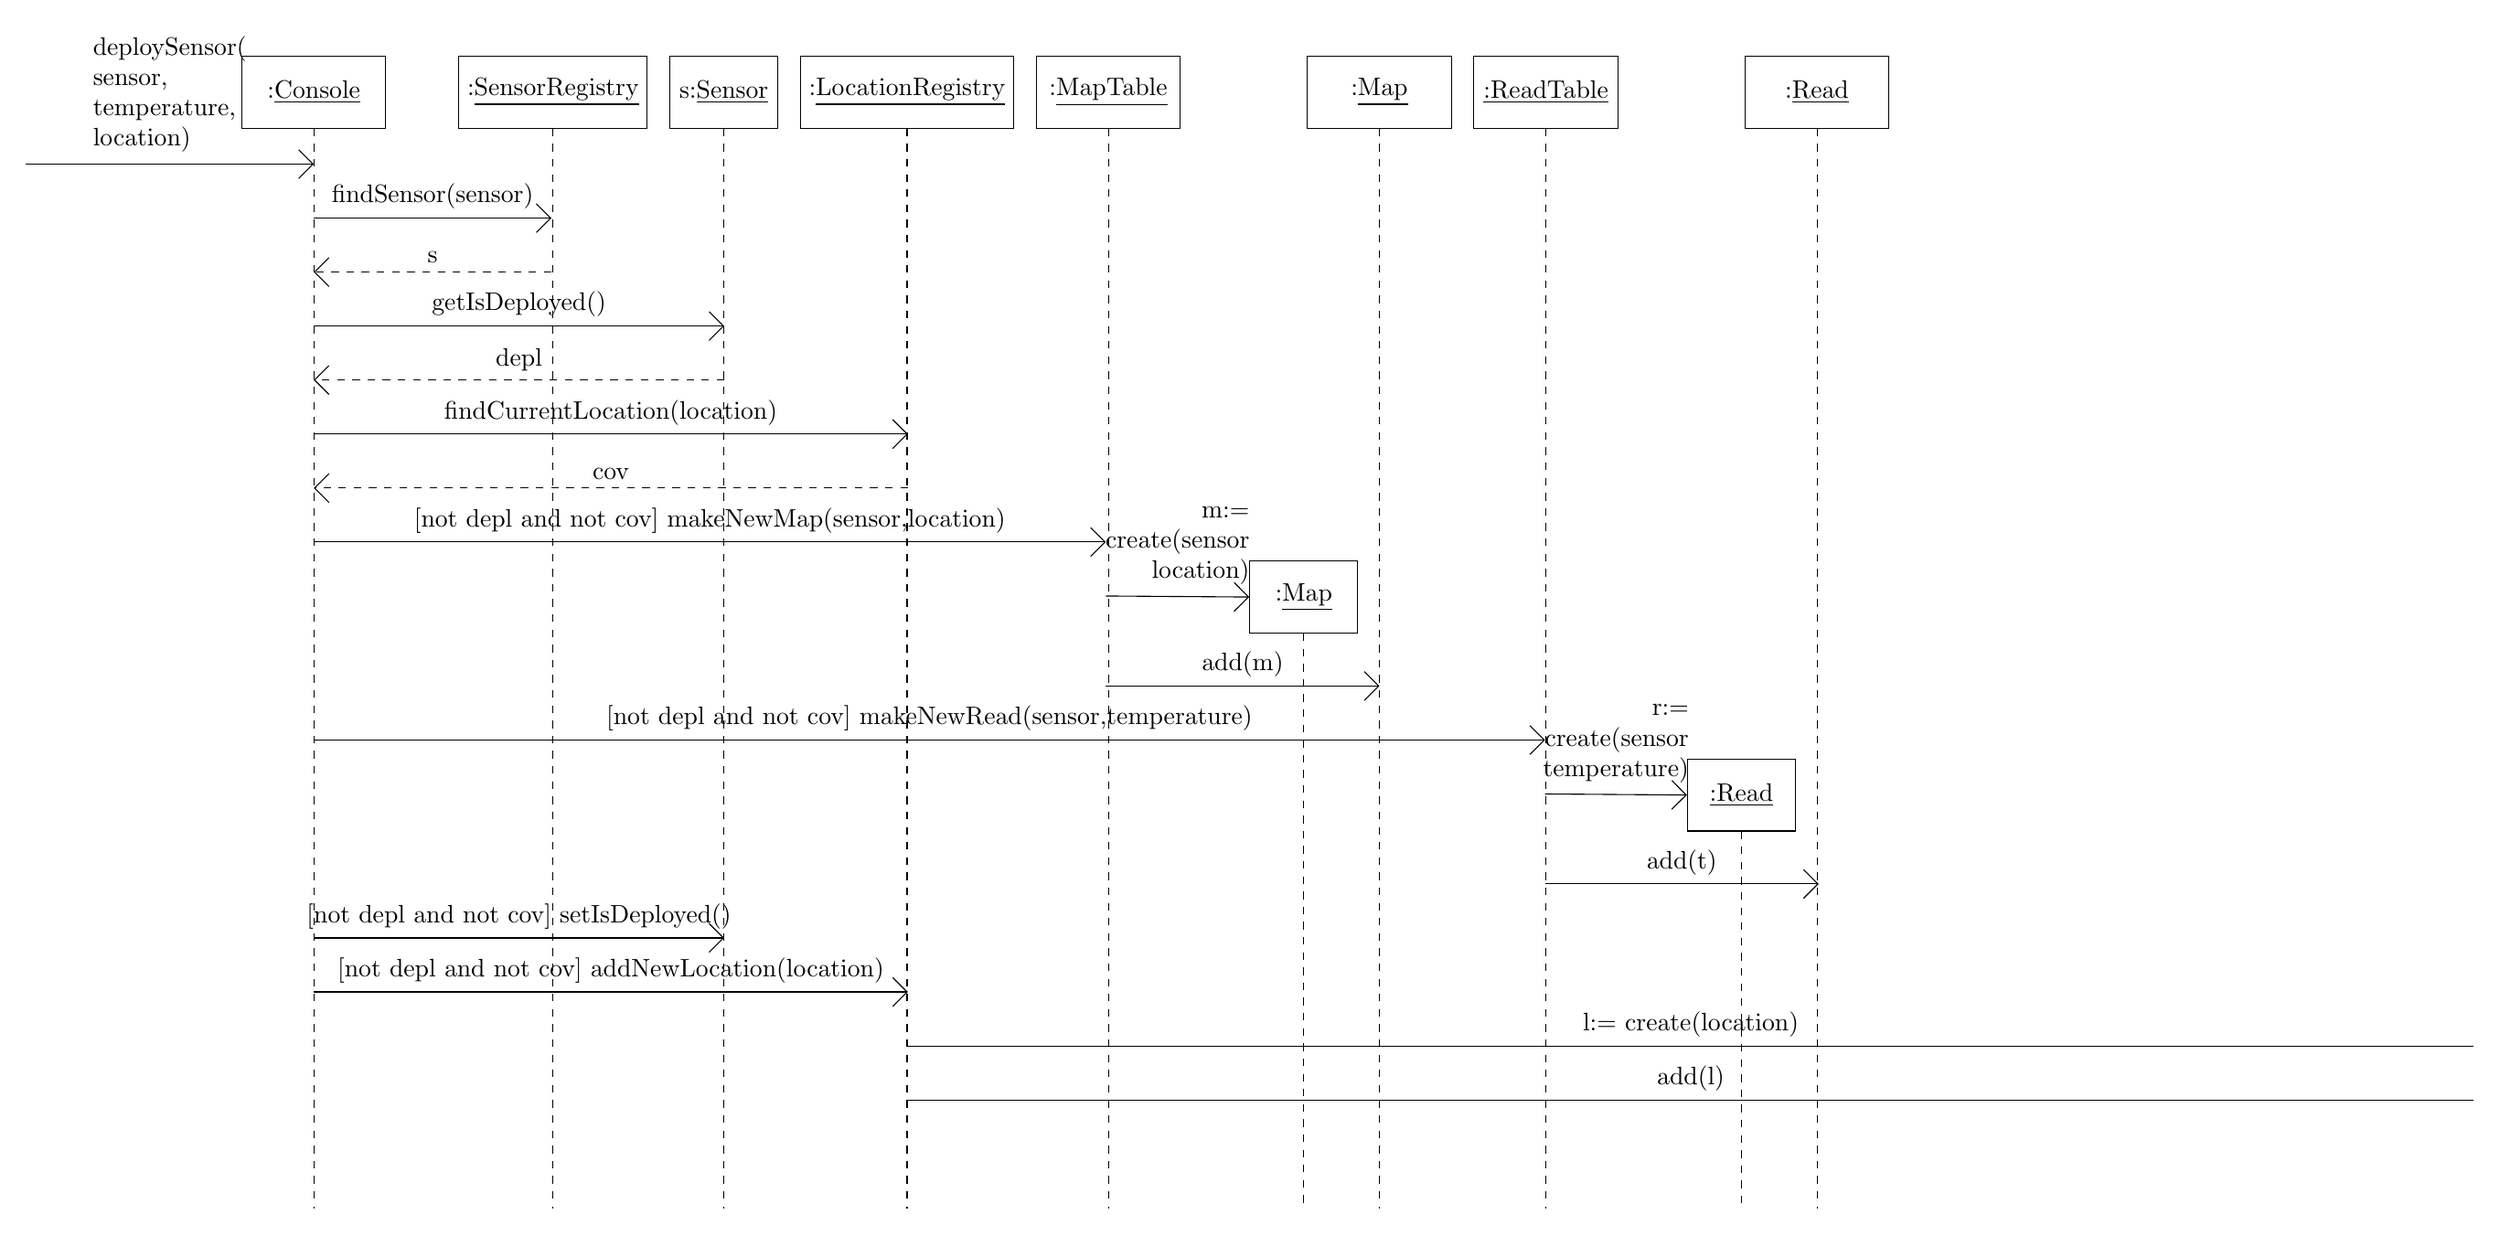
\begin{tikzpicture}[node distance=3cm]
	% --- Lifelines ---
	
	% Console
	\node[rectangle, draw, minimum width=2cm, minimum height=1cm, align=center] (console) {:\underline{Console}};
  \draw[dashed] (console.south) -- +(0,-15cm);
  
  	% Sensor Registry
  	\node[rectangle, draw, minimum width=2cm, minimum height=1cm, align=center, right=1cm of console] (sreg) {:\underline{SensorRegistry}};
  	\draw[dashed] (sreg.south) -- +(0,-15cm);
  	
  	% Sensor
  	\node[rectangle, draw, minimum width=1.5cm, minimum height=1cm, align=center, right=0.3cm of sreg] (sensor) {s:\underline{Sensor}};
  	\draw[dashed] (sensor.south) -- +(0,-15cm);
  	
  	% Location Registry
  	\node[rectangle, draw, minimum width=2cm, minimum height=1cm, align=center, right=0.3cm of sensor] (lreg) {:\underline{LocationRegistry}};
  	\draw[dashed] (lreg.south) -- +(0,-15cm);
  	
  	% Location
  	%\node[rectangle, draw, minimum width=2cm, minimum height=1cm, align=center, right=0.3cm of lreg] (loc) {l:\underline{Location}};
  	%\draw[dashed] (loc.south) -- +(0,-15cm);
  	
  	% Map Table
  	\node[rectangle, draw, minimum width=2cm, minimum height=1cm, align=center, right=0.3cm of lreg] (mapt) {:\underline{MapTable}};
  	\draw[dashed] (mapt.south) -- +(0,-15cm);
  	
  	% Map
  	\node[rectangle, draw, minimum width=1.5cm, minimum height=1cm, align=center, below right=6cm and 0.95cm of mapt] (map) {:\underline{Map}};
  	\draw[dashed] (map.south) -- +(0,-8cm);
  	
  	% Map List
  	\node[rectangle, draw, minimum width=2cm, minimum height=1cm, align=center, right=1.75cm of mapt] (mapl) {:\underline{Map}};
  	\draw[dashed] (mapl.south) -- +(0,-15cm);
  	
  	% Read Table
  	\node[rectangle, draw, minimum width=2cm, minimum height=1cm, align=center, right=0.3cm of mapl] (readt) {\underline{:ReadTable}};
  	\draw[dashed] (readt.south) -- +(0,-15cm);
  	
  	% Read
  	\node[rectangle, draw, minimum width=1.5cm, minimum height=1cm, align=center, below right=8.75cm and 0.95cm of readt] (read) {\underline{:Read}};
  	\draw[dashed] (read.south) -- +(0,-5.25cm);
  	
  	% Read List
  	\node[rectangle, draw, minimum width=2cm, minimum height=1cm, align=center, right=1.75cm of readt] (readl) {:\underline{Read}};
  	\draw[dashed] (readl.south) -- +(0,-15cm);
  	
  % --- Messages and calls ---
  \draw[-{Straight Barb[length=2mm]}] (-4, -1) -- (0, -1) node[midway, above] {%
\begin{tabular}{l}
deploySensor( \\
sensor, \\
temperature, \\
location)
\end{tabular}
};
  % Console and Sensor Registry
  \draw[-{Straight Barb[length=2mm]}] (0, -1.75) -- (3.3, -1.75) node[midway, above] {findSensor(sensor)};
  
  \draw[dashed, -{Straight Barb[length=2mm]}] (3.3, -2.5) -- (0, -2.5) node[midway, above] {s};
  
  % Console and Sensor
  \draw[-{Straight Barb[length=2mm]}] (0, -3.25) -- (5.7, -3.25) node[midway, above] {getIsDeployed()};
  
  \draw[dashed, -{Straight Barb[length=2mm]}] (5.7, -4) -- (0, -4) node[midway, above] {depl};
  
  % Console and Location Registry
  \draw[-{Straight Barb[length=2mm]}] (0, -4.75) -- (8.25, -4.75) node[midway, above] {findCurrentLocation(location)};
  
  % Location
  %\draw[-{Straight Barb[length=2mm]}] (8.25, -5.5) -- (11, -5.5) node[midway, above] {contains()};
  
  \draw[dashed, -{Straight Barb[length=2mm]}] (8.25, -5.5) -- (0, -5.5) node[midway, above] {cov};
  
  % Console, Map Table and Map  
  \draw[-{Straight Barb[length=2mm]}] (0, -6.25) -- (11, -6.25) node[midway, above] {[not depl and not cov] makeNewMap(sensor,location)};
  
  \draw[-{Straight Barb[length=2mm]}] (11, -7) -- (map.west) node[midway, above] {%
\begin{tabular}{r}
m:= \\
create(sensor \\
location)
\end{tabular}
};

  \draw[-{Straight Barb[length=2mm]}] (11, -8.25) -- (14.8,-8.25) node[midway, above] {add(m)};
  
  \draw[-{Straight Barb[length=2mm]}] (0, -9) -- (17.1, -9) node[midway, above] {[not depl and not cov] makeNewRead(sensor,temperature)};
  
  \draw[-{Straight Barb[length=2mm]}] (17.1, -9.75) -- (read.west) node[midway, above] {%
\begin{tabular}{r}
r:= \\
create(sensor \\
temperature)
\end{tabular}
};

  \draw[-{Straight Barb[length=2mm]}] (17.1, -11) -- (20.9,-11) node[midway, above] {add(t)};
  
  \draw[-{Straight Barb[length=2mm]}] (0, -11.75) -- (5.7,-11.75) node[midway, above] {[not depl and not cov] setIsDeployed()};
  
  \draw[-{Straight Barb[length=2mm]}] (0, -12.5) -- (8.25,-12.5) node[midway, above] {[not depl and not cov] addNewLocation(location)};
  
  \draw[-] (8.25, -13.25) -- (30,-13.25) node[midway, above] {l:= create(location)};
  
  \draw[-] (8.25, -14) -- (30,-14) node[midway, above] {add(l)};
  
  
\end{tikzpicture}
    \caption{Interaction Diagram for deploySensor}
\end{figure}
}

\newpage % Start a new page

\afterpage{%
\begin{figure}

    \begin{tikzpicture}[node distance=3cm]
	% --- Lifelines ---
	% Location
	\node[rectangle, draw, minimum width=2cm, minimum height=1cm, align=center] (loc) at (10, -13.25)  {:\underline{Location}};
  	\draw[dashed] (loc.south) -- +(0,-4cm);
  
  
  	\draw[-{Straight Barb[length=2mm]}] (0, -13.25) -- (loc.west) node[midway, above] {l:= create(location)};
  
  	%\draw[-{Straight Barb[length=2mm]}] (0, -14) -- (10,-14) node[midway, above] {add(l)};
  
	\end{tikzpicture}
\end{figure}
}

\end{document}
